\chapter{Funzioni di attivazione}\label{chpt:5}
Le funzioni di attivazione sono un elemento fondamentale delle reti neurali, in quanto introducono la non-linearità nel modello, permettendo di apprendere relazioni complesse nei dati. Senza funzioni di attivazione, una rete neurale profonda sarebbe equivalente a una semplice trasformazione lineare.

\section{Vanishing Gradient Problem}
Uno dei problemi principali nell'addestramento delle reti neurali profonde è il \textbf{Vanishing Gradient Problem}, questo si verifica quando il gradiente diventa molto piccolo negli strati più profondi, il modello  dunque apprenderà molto lentamente o smette persino di imparare. Questo problema si verifica con funzioni di attivazione come la funzione \textbf{sigmoide} e la funzione \textbf{tangente iperbolica}. L'esito di queste funzioni porta a dei valori per la maggior parte, molto simili fra loro vicini al valore zero o al valore uno, e proprio a causa di questa polarizzazione e eccessiva vicinanza di valori, questo porta alle problematiche descritte precedentemente.

\begin{figure}[h]
    \centering
    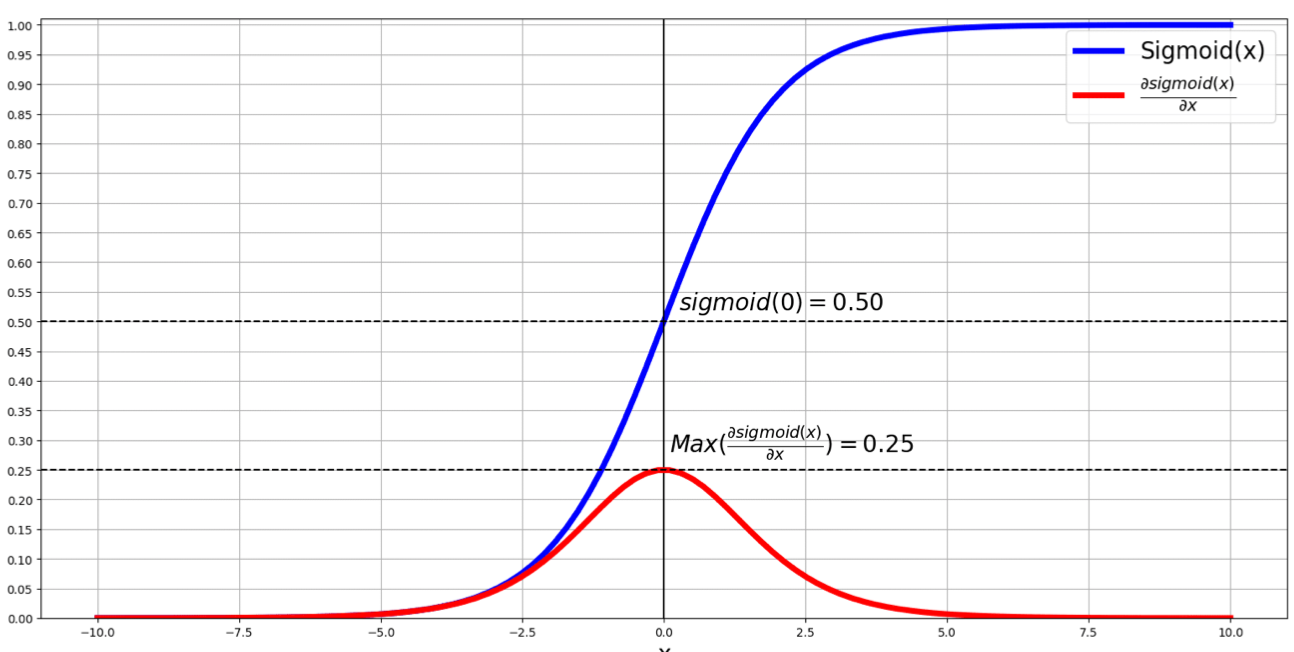
\includegraphics[width=0.85\textwidth]{figure/VanishingGradientProblem.png}
    \caption{Grafico descrittivo del Vanishing Gradient Problem, come possiamo vedere la derivata (in rosso) risulta essere molto ridotta per la gran parte dei valori.}
\end{figure}

\section{Funzioni non saturanti}
Per risolvere il problema dei gradienti che svaniscono, vengono utilizzate funzioni di attivazione \textbf{non-saturanti}, come:
\begin{itemize}
    \item \textbf{ReLU (Rectified Linear Unit)}: elimina i valori negativi rendendo i calcoli più efficienti, ma non risolve la problematica relativa al gradiente per i valori negativi, tuttavia ha un problema legato alla non derivabilità nel punto zero;
    \begin{equation}
        \operatorname{ReLU}(x) = \max(0, x)
    \end{equation}
    \item \textbf{Leaky ReLU}: introduce una piccola pendenza per i valori negativi, in modo tale da ridurre la problematica relativa a ciò che accadeva nel modello precedente;
    \begin{equation}
        \operatorname{LeakyReLU}(x) = \max(\alpha x, x)
    \end{equation}
    \item \textbf{PReLU (Parametric ReLU)}: simile a Leaky ReLU, ma il coefficiente della pendenza è appreso durante l'addestramento, pertanto posso avere anche una pendenza maggiore.
    \item \textbf{RReLU (Randomized ReLU)}: usa una pendenza casuale tramite l'uso di una variabile casuale nei valori negativi durante l'addestramento, mantenendo i sample in un range durante il traning, rimanendo poi fissato nel momento in cui si passa al testing.
\end{itemize}

\begin{figure}[h]
    \centering
    \begin{tikzpicture}
        \begin{axis}[xlabel={$x$}, ylabel={$f(x)$}, legend pos=north west, domain=-5:5, samples=100, grid]
            \addplot[color=deepblue, thick] {max(0,x)}; \addlegendentry{ReLU}
            \addplot[color=cadmiumorange, thick] {x >= 0 ? x : 0.01*x}; \addlegendentry{Leaky ReLU}
            \addplot[color=deepgreen, thick] {x >= 0 ? x : 0.1*x}; \addlegendentry{PReLU}
        \end{axis}
    \end{tikzpicture}
    \caption{Grafico di ReLU, Leaky ReLU e PReLU, tutti e tre i grafici dopo l'origine si sovrappongono, e seguono lo stesso andamento.}
\end{figure}

\section{Funzioni di Attivazione Avanzate}
Oltre a ReLU e le sue varianti, esistono altre funzioni di attivazione avanzate, queste puntano a risolvere il problema dell'appiattimento dei valori negativi e della non differenziabilità nel punto di coordinata zero:
\begin{itemize}
    \item \textbf{ELU (Exponential Linear Unit)}: permette valori negativi con una decrescita esponenziale, migliorando la stabilità.
    \item \textbf{SELU (Scaled ELU)}: usata per reti auto-normalizzanti.
    \item \textbf{GELU (Gaussian Error Linear Unit)}: si basa sulla distribuzione gaussiana per una transizione più fluida tra i valori.
    \item \textbf{Softplus}: una versione liscia della ReLU.
\end{itemize}

\begin{figure}[h]
    \begin{subfigure}{0.35\textwidth}
        \begin{tikzpicture}[scale=0.65]
            \begin{axis}[xlabel={$x$}, ylabel={$f(x)$}, domain=-5:5, samples=100,grid]
                \addplot[color=deepblue, thick] {x >= 0 ? x : (exp(x)-1)};
                \addplot[color=deepred, thick] {x >= 0 ? x : 1.05*(exp(x)-1)};
            \end{axis}
        \end{tikzpicture}
        \caption{ELU e SELU}
    \end{subfigure}
    \qquad\qquad\quad
    \begin{subfigure}{0.35\textwidth}
        \begin{tikzpicture}[scale=0.65]
            \begin{axis}[xlabel={$x$}, ylabel={$f(x)$}, domain=-5:5, samples=100,grid]
                \addplot[color=deepgreen, thick] {x >= 0 ? x : (exp(x)-1)};
                \addplot[color=cadmiumorange, thick] {0.5*x*(1+tanh(sqrt(2/pi)*(x+0.044715*x^3)))};
            \end{axis}
        \end{tikzpicture}
        \caption{CELU e GELU}
    \end{subfigure}
    \caption{Nel grafico sono rappresentate le varie funzioni di attivazione avanzate, a sinistra, vi è il confronto fra ELU (in blu) e SELU (in rosso), a destra invece il confronto fra CELU (in arancione) e GELU (in verde).}
\end{figure}

\section{Funzioni per la Normalizzazione}
\begin{itemize}
    \item \textbf{Hardtanh}: una versione limitata della tangente iperbolica, due valori costanti agli estremi e una retta obliqua che li collega centrata nell'origine.
    \item \textbf{Threshold}: taglia i valori al di sotto di una certa soglia, questa funzione di attivazione è stata la prima funzione di attivazione concepita fra gli anni '60 e gli anni '70.
    \item \textbf{Shrink Functions (Tanhshrink, Softshrink, Hardshrink)}: riducono progressivamente i valori verso zero.
\end{itemize}

\section{Funzioni Probabilistiche}
\begin{itemize}
    \item \textbf{Softmax}: questa funzione di attivazione trasforma un vettore in una distribuzione di probabilità all'interno di un range, essa inoltre enfatizza le differenze assegnando a valori più grandi una probabilità più alta, mentre quelli piccoli vengono schiacciati vicino allo zero, la somma di tutti i valori è pari a 1 ampliando la differenza fra i valori scalandoli a elementi dopo la virgola.
    \begin{equation}
        \operatorname{Softmax}(x_i) = \frac{e^{x_i}}{\sum_je^{x_j}}
    \end{equation}
    \item \textbf{Softmin}: la differenza rispetto alla Softmax è l'utilizzo del segno meno all'esponente. Questo fa sì che valori più piccoli abbiano un esponenziale più grande (quindi una probabilità maggiore), mentre i valori più grandi abbiano probabilità più piccole, essa inoltre è simmetrica rispetto al softmax.
    \begin{equation}
        \operatorname{Softmin}(x_i) = \frac{e^{-x_i}}{\sum_je^{-x_j}}
    \end{equation}
    \item \textbf{LogSoftmax}: quest'altra tipologia di funzione di attivazione invece è una variante della Softmax, in cui si applica il logaritmo alla funzione Softmax per migliorare la stabilità numerica e semplificare il calcolo della perdita nelle reti neurali.
    \begin{equation}
        \operatorname{LogSoftmax}(x_i) =\log( \frac{e^{x_i}}{\sum_je^{x_j}})
    \end{equation}
\end{itemize}

\begin{Osservazione}
    La softmax è facile notare come non sia altro che una generalizzazione della funzione sigmoide, poiché ci basta considerare il caso in cui ho due $x_i$ nel quale il secondo si annulla, e avrò in esito proprio la funzione sigmoide.
\end{Osservazione}
